%!TEX root = ../thesis.tex
%*******************************************************************************
%****************************** Third Chapter **********************************
%*******************************************************************************
\chapter{The Faser Experiment}

% **************************** Define Graphics Path **************************
\ifpdf
    \graphicspath{{ChapterFaser/Figs/Raster/}{Chapter3/Figs/PDF/}{Chapter3/Figs/}}
\else
    \graphicspath{{ChapterFaser/Figs/Vector/}{Chapter3/Figs/}}
\fi


\section{Experiment Location and Schedule}

\nomenclature[z-FASER]{FASER}{ForwArd Search ExpeRiment}                                % first letter Z is for Acronyms
\nomenclature[z-TAS]{TAS}{Target Absorbers}
\nomenclature[z-TAN]{TAN}{Target Absorber Neutral}
\nomenclature[z-LOS]{LOS}{Line Of Sight}

The FASER collaboration makes use of a disused tunnel, called TI12 (Fig. \ref{fig:infrastructure}), in just the right location to intercept these new particles that could be escaping from collisions in the ATLAS detector. The idea is that these light and weakly-interacting particles produced at the ATLAS IP will travel along the beam collision axis, unaffected by the magnets that bend the beams of particles around the ring of the LHC, through matter (mostly rock and concrete) without interacting and then interact within the FASER detector in TI12 \cite{faser_collaboration_faser:_2019}. The schedule is tight. The LHC is warmed up for maintenance until end of 2020, and FASER needs to be built before Run 3. A third long shutdown is planned for 2024 where the collaboration could do some maintenance/upgrade on FASER or install FASER 2, a bigger version of FASER.

In Fig. \ref{fig:infrastructure} we see that charged particles are deflected by the LHC magnets and that neutral hadrons are absorbed by either the Target Absorber for secondary particles (TAS) or Target Absorber Neutral (TAN) that are designed to protect the magnets. This means that only LLPs will travel from the IP to FASER through 10 meters of concrete and 90 meters of rock. In the SM only muons and neutrinos can reach FASER. However the LLPs is expected to easily pass through all of the material without interacting and then decay in FASER. We also see in the bottom right corner of Fig. \ref{fig:infrastructure} that FASER will be located roughly 5 meters from the LHC tunnel.

\begin{figure}[htbp!] 
\centering    
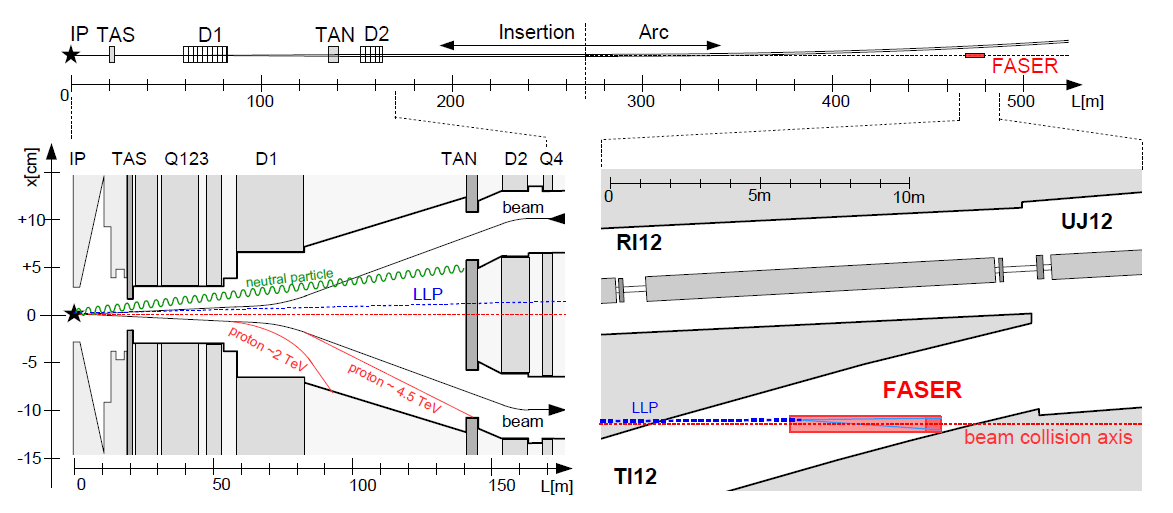
\includegraphics[width=1.0\textwidth]{FASERinfrastructureTI12.png}
\caption[TI12 Infrastructure]{TI12's infrastructure}
\label{fig:infrastructure}
\end{figure}

\subsection{Civil Engineering Work}

Some civil engineering work is needed to install the experiment in the tunnel. TI12 has a slight upwards slope which requires a trench to be cut out to align FASER with the beam collision axis. The digging depth will be around 50 cm and 5 m long. Figs. \ref{fig:TunnelBefore} and \ref{fig:TunnelAfter} show the civil engineering progress made in the tunnel.

\begin{figure}[htbp!] 
\centering
\begin{minipage}{.5\textwidth}
  \centering
  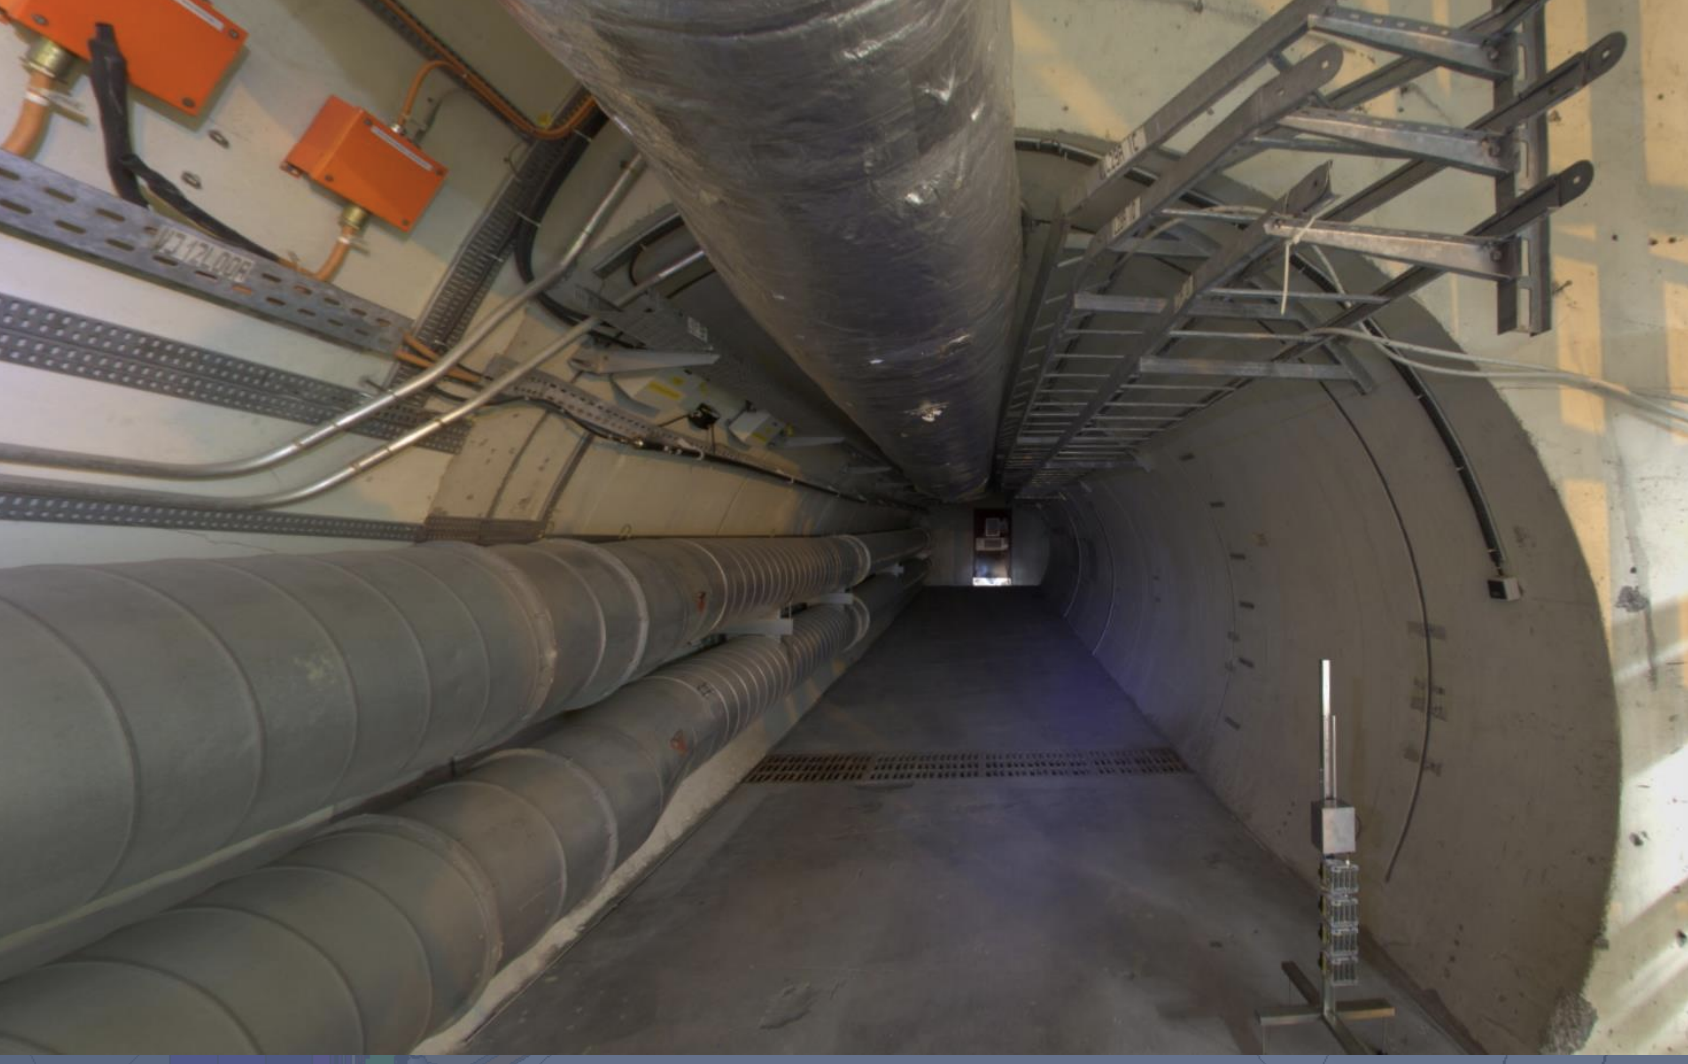
\includegraphics[width=.9\linewidth]{TunnelBefore}
  \captionsetup{width=0.8\textwidth}
  \caption[Unused TI12]{The disused TI12 tunnel before any accommodation for FASER.}
  \label{fig:TunnelBefore}
\end{minipage}%
\begin{minipage}{.5\textwidth}
  \centering
  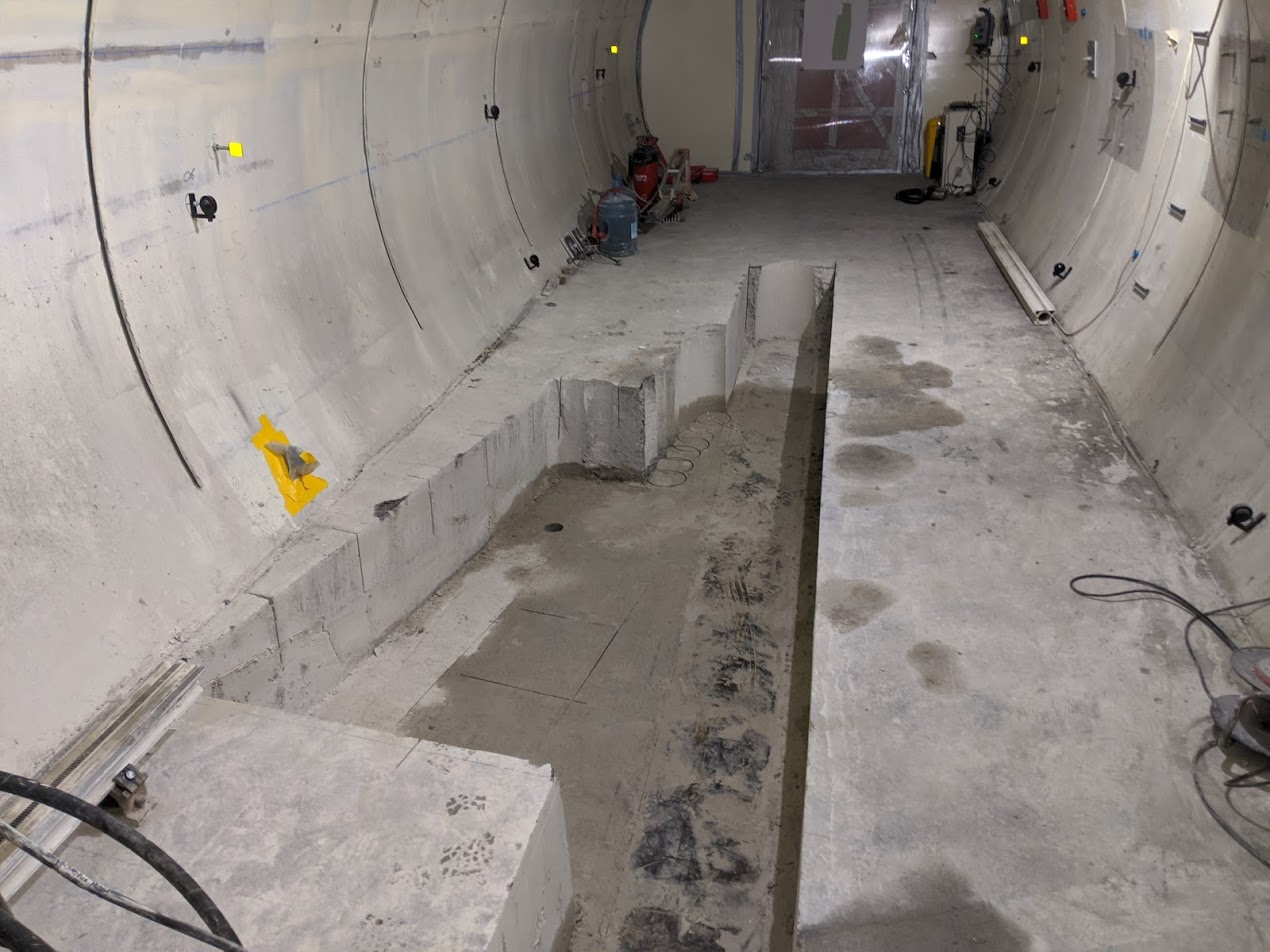
\includegraphics[width=.85\linewidth]{CEworks1.JPG}
  \captionsetup{width=0.8\textwidth}
  \caption[TI12 after civil engineering work]{Ventilation has been removed and a trench has been dug in preparation for the installation of the experiment.}
  \label{fig:TunnelAfter}
\end{minipage}
\end{figure}


\section{Magnet Design}

FASER will use a 0.6 T permanent dipole magnet made of neodymium iron boron (NdFeB), which unlike electromagnets does not require high voltage power or cooling. It will be thin enough to allow the line of sight to pass through the magnet centre with minimum digging in the floor of TI12. This is by far the most expensive piece of FASER. It will cost $\sim$450 kCHF, making up half the price of the experiment.

\begin{figure}[htbp!] 
\centering    
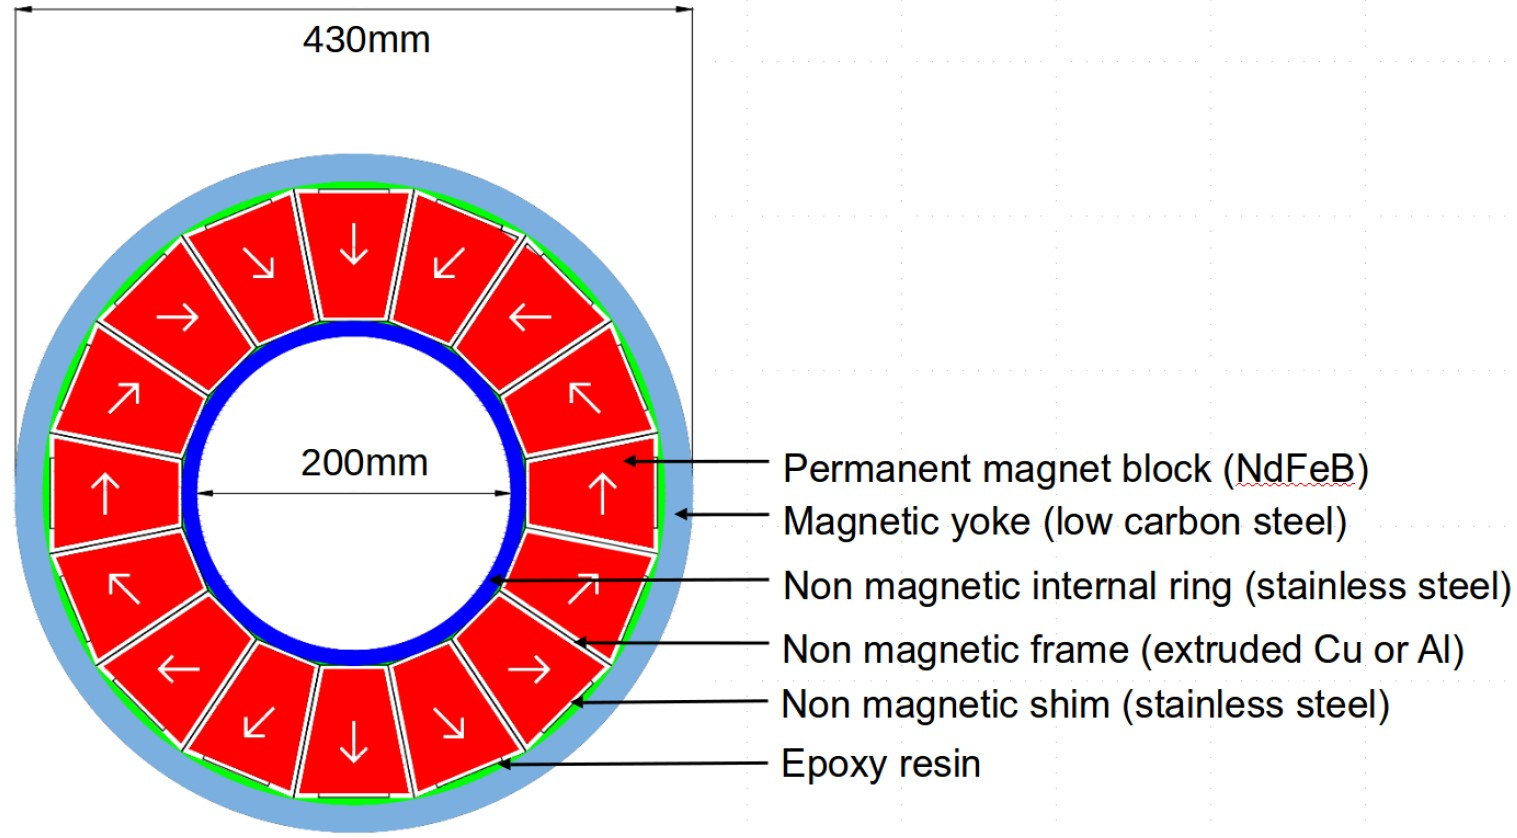
\includegraphics[width=0.6\textwidth]{ChapterFaser/Figs/Raster/MagnetDesign.jpg}
\caption[Magnet Design]{The magnet uses a Halbach array, a special arrangement of permanent magnets that augments the magnetic field on one side of the array while cancelling the field to near zero on the other side. This is achieved by having a spatially rotating pattern of magnetisation.
}
\label{fig:MagnetDesign}
\end{figure}

\section{Expected Signature}

\begin{figure}[htbp!] 
\centering    
    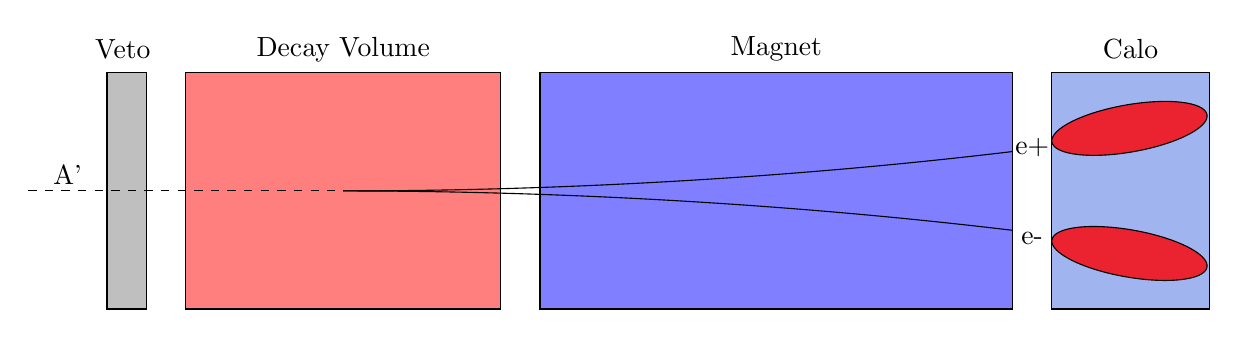
\begin{tikzpicture}
    \draw[fill=gray, fill opacity=0.5] (0,0) rectangle (0.5,3); %veto
    \draw[fill=red, fill opacity=0.5] (1,0) rectangle (5,3); %decay volume
    \draw[fill=blue, fill opacity=0.5] (5.5,0) rectangle (11.5,3); %magnet
    \draw[fill=RoyalBlue, fill opacity=0.5] (12,0) rectangle (14,3); %calo
    \node at (0.2,3.3) {Veto};
    \node at (3,3.3) {Decay Volume};
    \node at (8.5,3.3) {Magnet};
    \node at (13,3.3) {Calo};
    \draw[dashed] (-1,1.5) -- (3,1.5);
    \draw (3,1.5) parabola (11.5,2);
    \draw (3,1.5) parabola (11.5,1);
    \node at (-0.5,1.7) {A'};
    \node at (11.75,2.05) {e+};
    \node at (11.75,0.9) {e-};
    \draw[fill=red, fill opacity=0.8, rotate around={10:(13,2.5)}] (12.95,2.3) ellipse (1cm and 0.3cm);
    \draw[fill=red, fill opacity=0.8, rotate around={-10:(13,0.5)}] (12.95,0.7) ellipse (1cm and 0.3cm);
    \end{tikzpicture}    
\caption{Signal signature $A'\rightarrow e^{+}e^{-}$.}
\label{fig:SignalSignature}
\end{figure}

The long-lived particles that will travel and enter the 10 cm width of FASER will be highly energetic of the order of the TeV \cite{faser_collaboration_faser:_2019}. If we use that $p_{T}\sim m$:
\[ \theta\sim \frac{m}{E}\sim\frac{p_{T}}{E}\leq 1 \text{ mrad} \implies E\sim \text{TeV}\]
A characteristic signal event would be a long lived particle production after a $pp$ collision followed by the LLP's decay into TeV SM particles after the travel to FASER:
\[ pp \rightarrow \text{LLP} + \text{X}, \text{ LLP travels} \sim \text{480 m}, \text{ LLP} \rightarrow e^{+}e^{-}, \mu^{+}\mu^{-}, \pi^{+}\pi^{-},\gamma\gamma,\dots \]

\subsubsection{Signal signature $A'\rightarrow e^{+}e^{-}$}

A typical signature, shown in Fig. \ref{fig:SignalSignature}, for the $A'\rightarrow e^{+}e^{-}$ would be no signal in the veto scintillator and two high energy oppositely charged tracks, consistent with originating from a common vertex in the decay volume, and with a combined momentum pointing back to the IP. A large electromagnetic energy would be deposited in the calorimeter. The magnets are extremely important to separate the decay products of such light and highly energetic particles. Without them the decay products would only be separated by a few hundred $\mu$m after traveling 1 m in the detector. For a LLP with mass $\sim$ 100 MeV and energy $E\sim1$ TeV:

\[ \theta\sim\frac{m}{E}\sim\frac{100\,\text{MeV}}{1\,\text{TeV}}\sim100\,\mu\text{rad} \]
This is why the FASER magnets are needed to separate the tracks of the products.

\section{Detector Break Down}

\begin{figure}[htbp!] 
\centering    
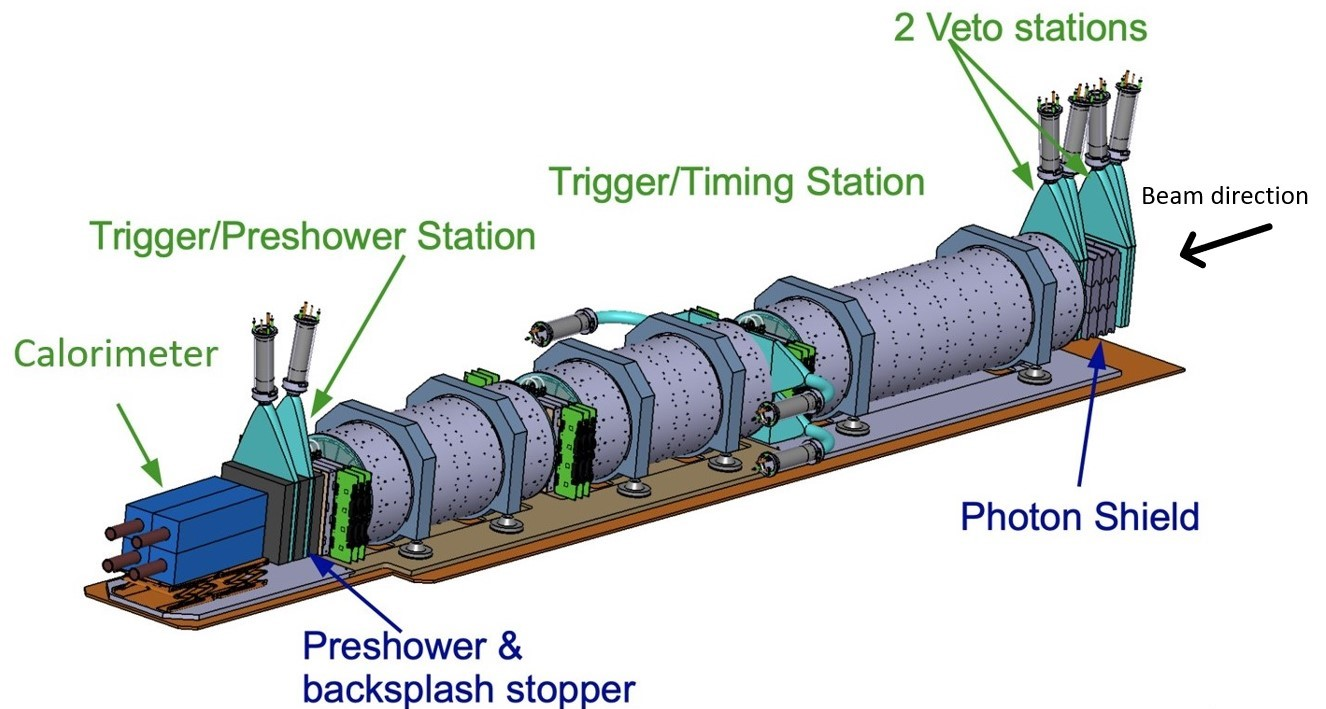
\includegraphics[width=0.8\textwidth]{ChapterFaser/Figs/Raster/FaserSchema.jpg}  
\caption{FASER Schematic.}
\label{fig:FaserSchematic}
\end{figure}

\begin{wrapfigure}{R}{0.3\textwidth}
  \centering
    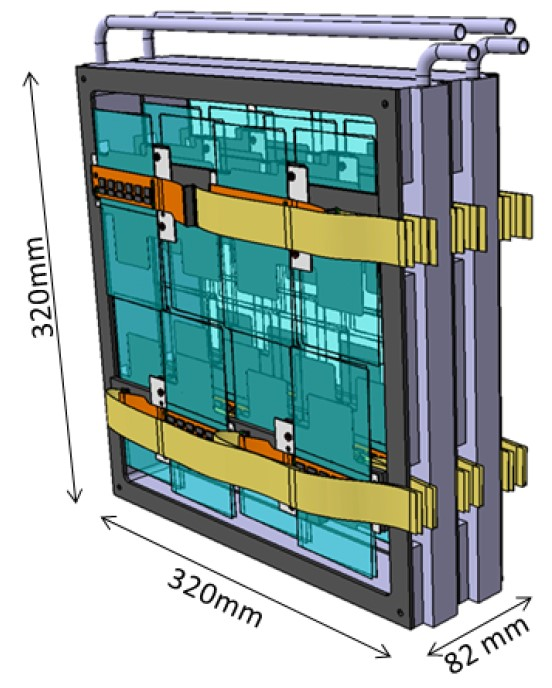
\includegraphics[width=0.28\textwidth]{ChapterFaser/Figs/Raster/TrackerStation.jpg} 
    \caption[Tracking Station]{One of the three Tracking Station.}
    \label{fig:TrackingStation}
\end{wrapfigure}

The FASER experiment is composed of multiple detectors, shown in Fig. \ref{fig:FaserSchematic}, that must all work in harmony to discover BSM particles. The beam first enters the front of the detector (right of Fig. \ref{fig:FaserSchematic}) composed of two scintillator stations that are used to veto charged particles, primarily high-energy muons, coming from the IP. Each of these station is made up of two layers of scintillators and has in between them a lead photon shield that converts photons into electromagnetic showers that can be vetoed by the scintillators. After the veto stations, the product of the particles decaying in the decay volume will be separated by the 1.5 m long magnet. The decay volume is followed by a spectrometer consisting of two 1 m long magnet and three tracking stations to reconstruct the path of the pair of charged particles and measure their momenta. At the entrance of and exit of the spectrometer are placed scintillator stations for triggering and precision time measurements. Finally, an electromagnetic calorimeter will identify high-energy electrons and photons and measure the total electromagnetic energy \cite{faser_collaboration_technical_2018}.

\subsection{Trackers}
The FASER tracker's purpose is to reconstruct the trajectories of energetic charged particles that will have decayed in the decay volume. The tracker will be made up of 3 tracking stations, shown on Fig. \ref{fig:TrackingStation}, located after each of the three magnet segments. Each of the tracking stations are composed of 3 layers, like the ones displayed in Fig. \ref{fig:TrackingLayer}, of double sided silicon strip detectors that each contain 8 SCT modules shown on Fig. \ref{fig:SCT}. All of the SCT modules used are spare modules previously used in the ATLAS experiment that allows the FASER collaboration to save 
resources \cite{faser_collaboration_technical_2018}.

\begin{figure}
\centering
\begin{minipage}[t]{.5\textwidth}
  \centering
  \captionsetup{width=0.8\textwidth}
    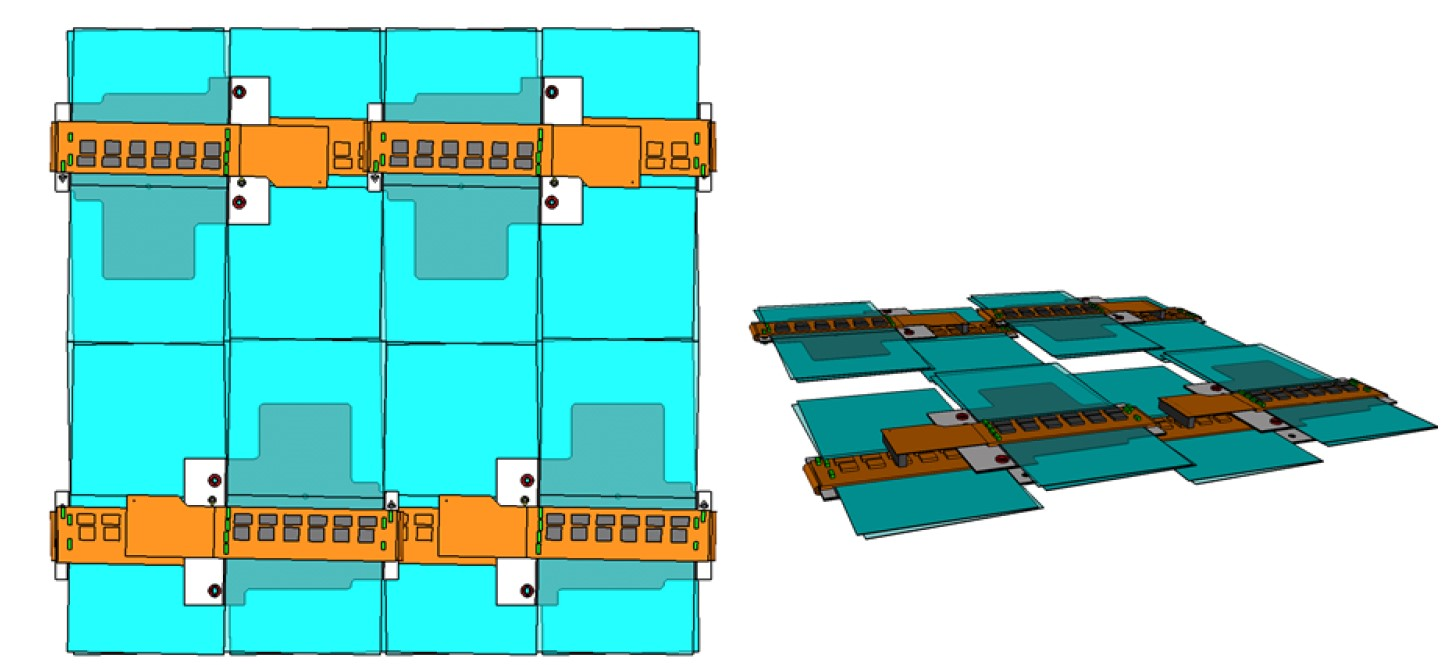
\includegraphics[width=0.9\textwidth]{ChapterFaser/Figs/Raster/TrackerLayer.jpg}  
    \caption[Tracking Layer]{A Tracking Layer. Each SCT module is 6 cm $\times$ 12 cm and the
    tracking plane is made of 8 modules, giving a square of about 24 cm $\times$  24 cm covering the full active area of the detector}
    \label{fig:TrackingLayer}
\end{minipage}%
\begin{minipage}[t]{.5\textwidth}
  \centering
  \captionsetup{width=0.8\textwidth}
    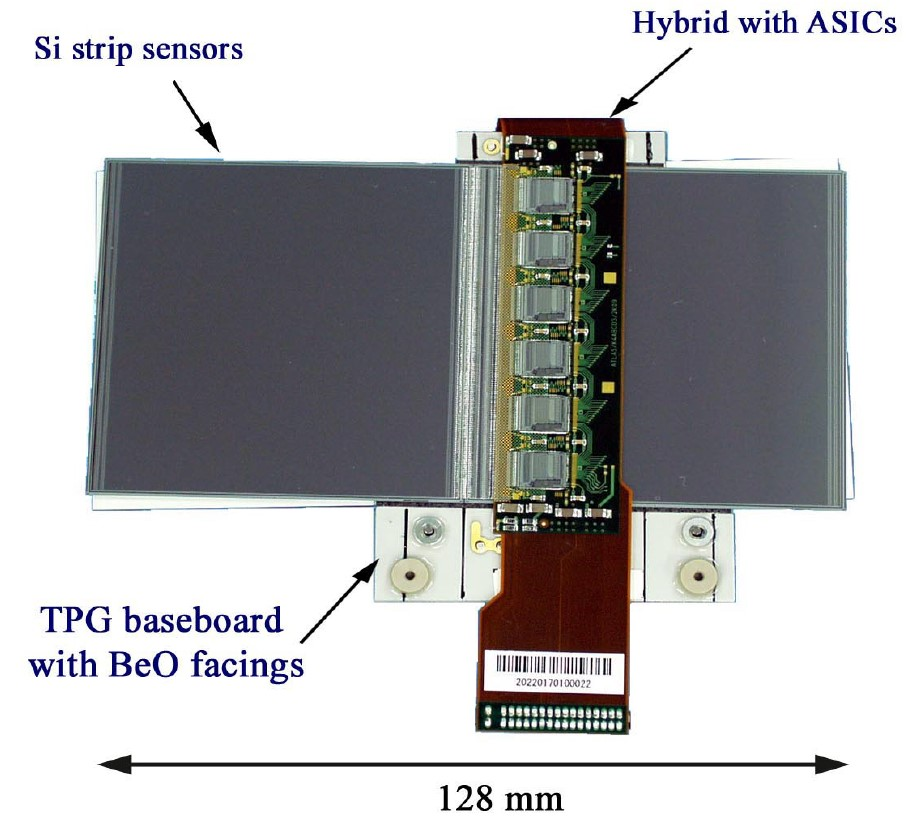
\includegraphics[width=0.9\textwidth]{ChapterFaser/Figs/Raster/SCT.jpg}  
    \caption[SCT Module]{An SCT Module. Visible in the middle are 6 of the 12 on-board ASIC chips that must be actively cooled with a water loop.}
    \label{fig:SCT}
\end{minipage}
\end{figure}

\subsection{Calorimeter}

The calorimeter installed at the back of FASER will measure the electromagnetic energy of the event. It will be able to identify electrons and photons and will be used for triggering. As for the Tracker, the calorimeter will use 4 spare LHCb outer ECAL modules.
It is composed of 66 layers of lead/scintillator that are readout by photomultiplers (PMTs) (no longitudinal shower information). Its dimensions are 12cm $\times$ 12cm – 75cm long (including PMT) and provides $\sim$ 1\% energy resolution for 1 TeV electrons. However, the resolution will degrade at higher energy due to not containing full shower in calorimeter.

\subsection{Scintillators}

Scintillators will be used to identify charged particles entering the decay volume, and for triggering. They will use PMT for the readout. They are produced at CERN and are capable of extremely efficient charged particle veto.\\
Eight scintillators will be used in FASER. A double layer of scintillators, shown in Fig. \ref{fig:ScintillatorSchema}, will be located at the entrance of the detector to veto incoming charged particles, primarily high-energy muons followed by a thick layer of lead converting photons into electromagnetic shower that can be efficiently vetoed by an additional double layer of scintillator.\\
After the first magnet and tracking layer is located the timing/trigger station composed of a double layer of wider scintillators, see Fig. \ref{fig:Scintillator2Schema}. They are used to detect the first appearance of a charged particle pair from the decay of an LLP in the decay volume. It will be used as the primary trigger and to measure time elapsed since the proton-proton collision at the IP.\\
A final scintillators station is located in front of the calorimeter. It is used to provide an additional trigger that can be used in tandem with the first one and has a thin layer of material (either tungsten or lead) in front of it to create a simple preshower detector. This will allow the detection of the physics signal of two close-by energetic photons
 \cite{faser_collaboration_technical_2018}.

\begin{figure}[htbp!] 
\centering    
    \begin{tikzpicture}
    \draw[fill=Periwinkle!30] (0,0) rectangle (3,3); %square
    \fill[fill=Periwinkle!30] (3,3)--(6,1.7)--(6,1.3)--(3,0); %light guide
    \draw[] (3,3)--(6,1.7);
    \draw[] (6,1.7)--(6,1.3);
    \draw[] (6,1.3)--(3,0);
    \draw[] (3,0)--(3,3);
    \shade[top color=Periwinkle!20,bottom color=CadetBlue!80] (6,1.7) rectangle (6.1,1.3);%small intersection piece
    \draw[] (6,1.7)--(6.1,1.7);
    \draw[] (6.1,1.7)--(6.1,1.3);
    \draw[] (6.1,1.3)--(6,1.3);
    \draw[] (6,1.3)--(6,1.7);
    \shade[top color=Periwinkle!20,bottom color=CadetBlue!80] (6.1,1.8) rectangle (7,1.2);%big intersection piece
    \draw[] (6.1,1.8)--(7,1.8);
    \draw[] (7,1.8)--(7,1.2);
    \draw[] (7,1.2)--(6.1,1.2);
    \draw[] (6.1,1.2)--(6.1,1.8);
    \shade[top color=Brown!20,bottom color=Brown] (7,1.75) rectangle (9,1.25);%PMT
    \draw[] (7,1.75)--(9,1.75);
    \draw[] (9,1.75)--(9,1.25);
    \draw[] (9,1.25)--(7,1.25);
    \draw[] (7,1.25)--(7,1.75);
    % Dimensions
    \draw[] (-0.4,0)--(-1,0);
    \draw[] (-0.4,3)--(-1,3);
    \draw[>=triangle 45, <->] (-0.7,0)--(-0.7,3);
    \draw[] (0,3.4) -- (0,4);
    \draw[] (3,3.4) -- (3,4);
    \draw[>=triangle 45, <->] (0,3.7) -- (3,3.7);
    \node at (1.5,4) {30 cm};
    \node[rotate=90] at (-1,1.5) {30 cm};
    \node at (4.3,1.5) {Light Guide};
    \node at (8,2.1) {PMT};
    \end{tikzpicture}    
\caption[Scintillator schema]{Six of these scintillators will be used for the veto and preshower stations. The basic design is 2 cm-thick, 30 cm $\times$ 30 cm
plastic scintillator made of Bicron connected through a light guide to a Hamamatsu H3178-51 PMT.}
\label{fig:ScintillatorSchema}
\end{figure}

\begin{figure}[htbp!] 
\centering    
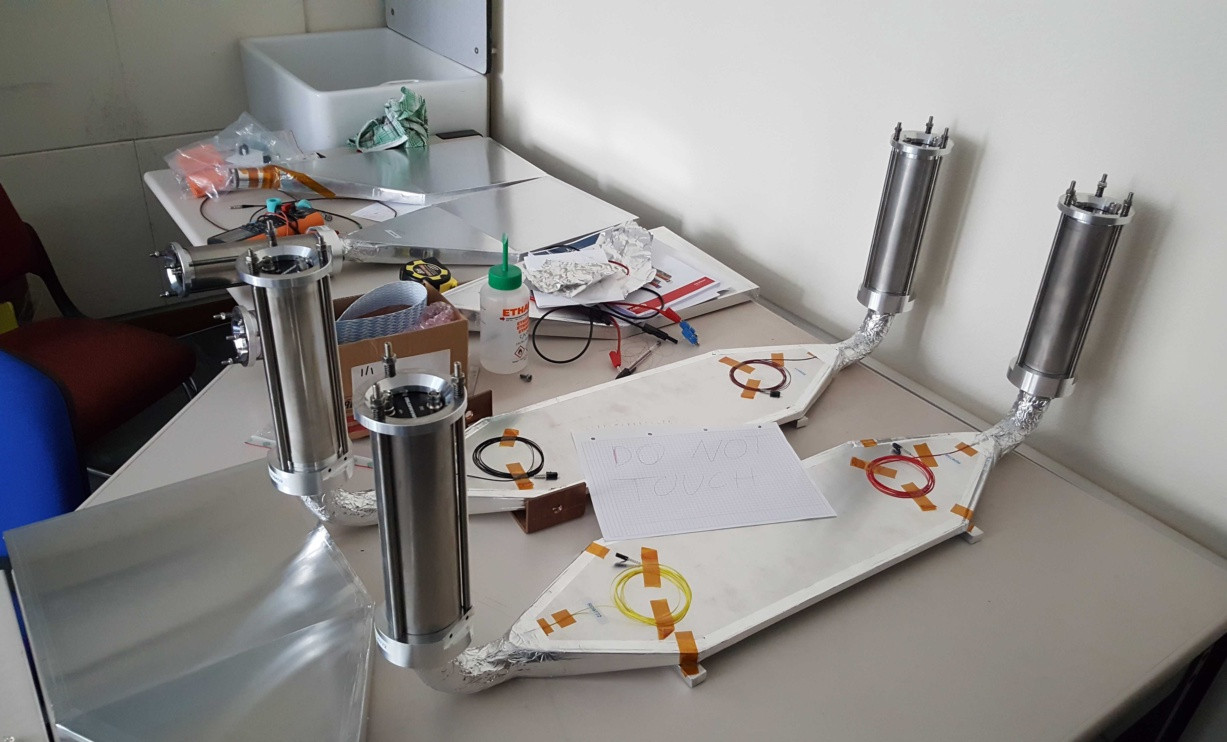
\includegraphics[width=0.7\textwidth]{ChapterFaser/Figs/Raster/doublescint.jpeg}  
\caption[Scintillator used for timing/trigger]{Scintillators used for the timing/trigger station. Their dimension are 1 cm-thick, 20 $\times$ 40 cm. Because they are wider, PMTs have been installed on both sides. Two scintillators will be offset along the line of sight to introduce an overlap and avoid inefficiency.}
\label{fig:Scintillator2Schema}
\end{figure}